\section{Erfaring}
En samlet liste af erfaringen de to kandidater har indenfor feltet hyttebombing indenfor Polyteknisk Forening:

\subsection{Studiestarten}
\begin{enumerate}
\item Vektor 2006
\item CSK 2007
\item CSK 2008
\item Vektor 2008
\item CSK 2009
\item Vektor 2009
\end{enumerate}

\subsection{Madhold}
\begin{enumerate}
\item vOPtur 2008
\item Rustur 2009
\item hyttetur ELKO nystartende 2010
\item S-husets hyttetur 2011
\item OPtur 2011
\item Rustur 2011
\item hyttetur ELKO nystartende 2011
\item S-husets hyttetur 2012
\end{enumerate}


\subsection{Arrangør af ture}

\begin{enumerate}
\item Rustur 2006
\item HerreHyggeHyttetur ELKO 2007 
\item OPtur 2007
\item Rustur 2007
\item HerreHyggeHyttetur ELKO 2008
\item OPtur 2008
\item Rustur 2008
\item hyttetur ELKO nystartende 2008
\item HerreHyggeHyttetur ELKO 2009
\item OPtur 2009
\item Rustur 2009
\item hyttetur ELKO nystartende 2009
\item HerreHyggeHyttetur ELKO 2011
\item HerreHyggeHyttetur ELKO 2012
\end{enumerate}

\subsection{PF kompetancer}
\begin{enumerate}
\item Medlem ELKO 2006-2012
\item Formand for ELKO rådet 2007-2009
\item UddanelsesPolitisk Råd 2007-2012
\item ISN Fotonik 2007-2012
\item Hegnet 2007->
\item Hegnet Formand 2007-2008
\item Fællesrådet 2009+2011-2012
\item Fællesrådets ForretningsUdvalg 2009-2012
\item PF's Bestyrelse 2010
\item Formand for ELKO rådet 2011-2012
\item Akademisk Råd (DTU) 2011-2012
\end{enumerate}

\section{Kødpopularitet}


%\begin{tikzpicture}
%\begin{axis}[
%ybar,
%enlargelimits=0.15,
%legend style={at={(0.5,-0.15)},
%anchor=north,legend columns=-1},
%ylabel={\#participants},
%symbolic x coords={tool8,tool9,tool10},
%xtick=data,
%nodes near coords,
%nodes near coords align={vertical},
%]
%\addplot coordinates {(tool8,7) (tool9,9) (tool10,4)};
%\addplot coordinates {(tool8,4) (tool9,4) (tool10,4)};
%\addplot coordinates {(tool8,1) (tool9,1) (tool10,1)};
%\legend{used,understood,not understood}
%\end{axis}
%\end{tikzpicture}
Herunder er de mest gængse kødprodukter listet efter popularitet i følge En unavngiven kilde der følger miljøet tæt:

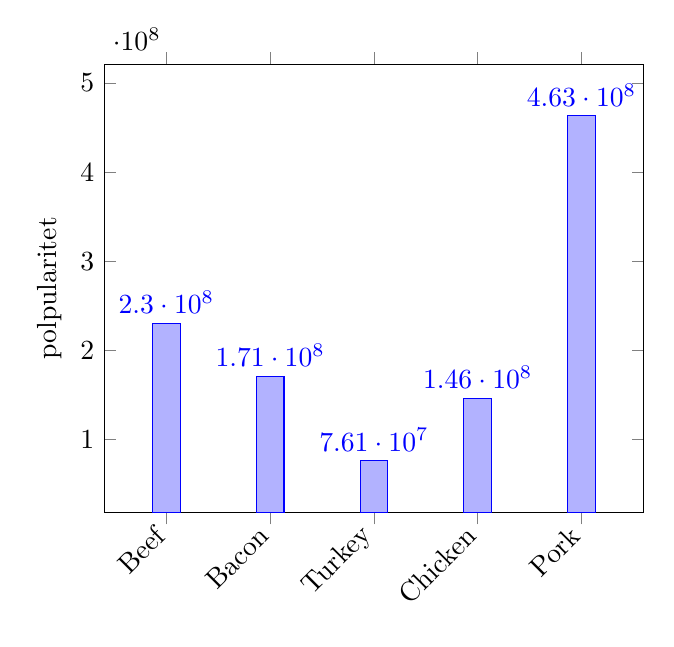
\begin{tikzpicture}
\begin{axis}[
ybar,
enlargelimits=0.15,
legend style={at={(0.5,-0.1)},
anchor=north,legend columns=-1},
ylabel={polpularitet},
symbolic x coords={Beef,	Bacon,	Turkey,	Chicken,	Pork},
xtick=data,
nodes near coords,
nodes near coords align={vertical},
x tick label style={rotate=45,anchor=east},
]
\addplot coordinates {(Beef,230000000) (Bacon,171000000) (Turkey,76100000) (Chicken,146000000) (Pork,463000000)};
\end{axis}
\end{tikzpicture}

En nærmere undersøgelse viser dog tydeligt Bacons posistion som svinets mest elskede kød:
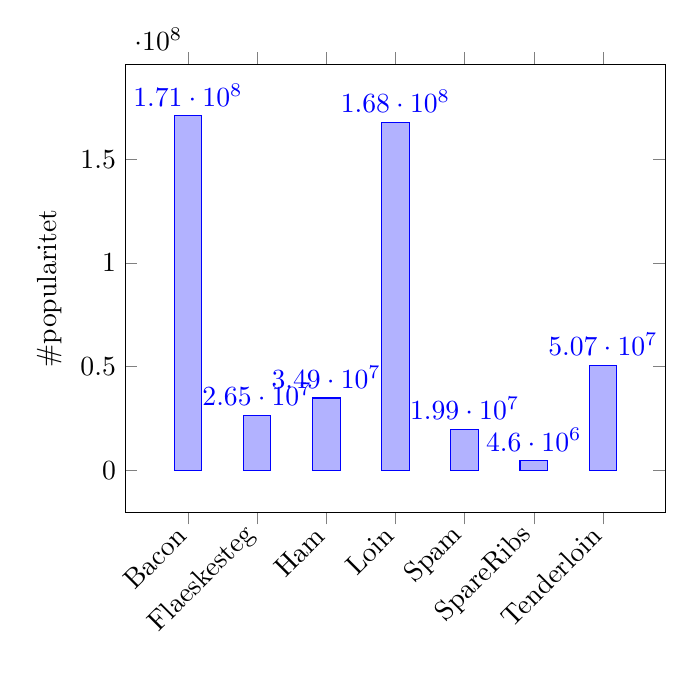
\begin{tikzpicture}
\begin{axis}[
ybar,
enlargelimits=0.15,
legend style={at={(0.5,-0.2)},
anchor=north,legend columns=-1},
ylabel={\#popularitet},
symbolic x coords={Bacon,Flaeskesteg,Ham,Loin,Spam,SpareRibs,Tenderloin},
xtick=data,
nodes near coords,
nodes near coords align={vertical},
x tick label style={rotate=45,anchor=east},
]
\addplot coordinates {(Bacon,171000000) (Flaeskesteg,26500000) (Ham,34900000) (Loin,168000000) (Spam,19900000)(SpareRibs,4600000)(Tenderloin,50700000)};
\end{axis}
\end{tikzpicture}

SPAM\footnote{Well, there's egg and bacon; egg sausage and bacon; egg and spam; egg bacon and spam; egg bacon sausage and spam; spam bacon sausage and spam; spam egg spam spam bacon and spam; spam sausage spam spam bacon spam tomato and spam; spam spam spam egg and spam; spam spam spam spam spam spam baked beans spam spam spam or Lobster Thermidor a Crevette with a mornay sauce served in a Provencale manner with shallots and aubergines garnished with truffle pate, brandy and with a fried egg on top and spam.}



\section{Hvad er Tha Bombs ikke}
\begin{enumerate}
\item Pædofil \cite{bib:url:Finn:Pedo}
\item Satan-tilbeder \cite{bib:url:Finn:Satan}
\item Dyrker sex med sovende kvinder \cite{bib:url:Finn:SovendeKvinder}
\item TV2 ansat \cite{bib:url:Finn:TV2}
\item Nazist\cite{bib:url:Finn:Nazist}
\end{enumerate}


Vi skal bruger DILD\cite{bib:url:Reklame:Dild}
\\
\\
Vi skal have en Anit Jehova Pæl \cite{bib:url:Reklame:Anti}
\\
\\
Tun i vand skal bruges \cite{bib:url:Reklame:Tun} rigeligt med tun i vand
\\
\\

